
\chapter{Data Restoration on the Sphere}
\label{ch_restore}
\index{Denoising}
\index{Filtering}

\label{sect_exp}
\section{Introduction}
\index{wavelet!denoising}
\index{curvelet!denoising}

Wavelets and Curvelets have been used successfully for image denoising via non-linear filtering or 
thresholding methods \citep{starck:book06,starck:book10}. Hard thresholding, for instance, consists in 
setting all insignificant coefficients (i.e. coefficients with an absolute value below a given 
threshold) to zero. In practice, we need to estimate the noise standard deviation $\sigma_j$ in each band 
$j$ and a wavelet (or curvelet) coefficient $w_j$ is significant if $\mid w_j \mid > k \sigma_j$, where $k$ 
is a user-defined parameter, typically chosen between 3 and 5. The $\sigma_j$ estimation in band $j$ can be 
derived from simulations \citep{starck:book06}. Denoting $D$ the noisy data and $\delta$ the thresholding 
operator, the filtered data $\tilde D$ are obtained by : 
\begin{eqnarray}
 {\tilde D} =    {\cal R} \delta( {\cal T} D)
\end{eqnarray}
where ${\cal T}$ is the wavelet (resp. curvelet) transform operator and ${\cal R}$ is the wavelet (resp. curvelet) reconstruction operator. 

\section{Significant Wavelet Coefficients}
\label{ch_noise}
\subsection{Definition}
\index{noise}
\index{wavelet!significant coefficient}

In most applications, it is necessary to know if a wavelet coefficient is due to signal (i.e.\ it is significant) or to noise. 

The wavelet (resp. curvelet) transform yields a set of resolution-related views of the input image. 
A wavelet (resp. curvelet) band at level $j$ has coefficients given by $w_{j,k}$. If we obtain the 
distribution of the coefficient $w_{j,k}$ for each band of the decomposition, based on the noise, 
we can introduce a statistical significance test for this coefficient. This procedure is the classical 
significance-testing one. Let ${\cal H}_0$ be the hypothesis that the image is locally constant at scale $j$.  
Rejection of hypothesis ${\cal H}_0$ depends (for positive coefficient values) on:
\begin{eqnarray}
P = Prob(\mid w_{j,k} \mid \ < \ \tau \mid {\cal H}_0)  
\end{eqnarray}
The detection threshold, $\tau$, is defined for each scale. Given an estimation threshold, $\epsilon$, 
if $P = P(\tau) > \epsilon$ the null hypothesis is not excluded. Although non-null, the value of the 
coefficient could be due to noise. On the other hand, if $P < \epsilon$, the coefficient value cannot be due to 
the noise alone, and so the null hypothesis is rejected. In this case, a significant coefficient has been detected.

\subsection{Noise Modeling}
\index{noise}
\index{noise!Gaussian}
If the distribution of $w_{j,l}$ is Gaussian, with zero mean and standard deviation $\sigma_j$, we have the probability density
\begin{eqnarray}
p(w_{j,l}) = \frac{1}{\sqrt{2\pi} \sigma_j} e^{{- w_{j,l}^2}/2\sigma^2_j} 
\end{eqnarray}
Rejection of hypothesis ${\cal H}_0$ depends (for a positive coefficient value) on:
\begin{eqnarray}
P = Prob( w_{j,l} > W) = \frac{1}{\sqrt{2\pi} \sigma_j} \int^{+\infty}_{w_{j,l}} e^{-W^2/2\sigma^2_j} dW 
\end{eqnarray}
and if the coefficient value is negative, it depends on 
\begin{eqnarray}
P = Prob( w_{j,l} < W) = \frac{1}{\sqrt{2\pi} \sigma_j} \int^{w_{j,l}}_{-\infty} e^{-W^2/2\sigma^2_j} dW 
\end{eqnarray}

Given stationary Gaussian noise, it suffices to compare $w_{j,l}$ to 
\index{stationary signal}
$k \sigma_j$.  Often $k $ is chosen as 3, which corresponds approximately to $\epsilon = 0.002$.  
If $w_{j,l}$ is small, it is not significant and could be due to noise. If $w_{j,l}$ is large, it is significant:
\begin{eqnarray}
\begin{array}{l}
\mbox{ if }  \mid  w_{j,l} \mid \ \geq \ k \sigma_j \ \ \mbox{ then } w_{j,l}   \mbox{ is significant } \\ 
\mbox{ if }  \mid  w_{j,l} \mid \ < \ k \sigma_j \ \ \mbox{ then }  w_{j,l} \mbox{ is not significant }
\end{array}
\end{eqnarray}

So we need to estimate, in the case of Gaussian noise models, the noise standard deviation at each scale. 
These standard deviations can be determined analytically, but the calculations can become complicated.  

The appropriate value of $\sigma_j$ in the succession of wavelet planes is assessed from the standard deviation 
of the noise $\sigma_N$ in the original data $D$, and from study of the noise in the wavelet space. This study 
consists of simulating a data set containing Gaussian noise with a standard deviation equal to 1, and taking the 
wavelet transform of this data set. Then we compute the standard deviation $\sigma^e_j$ at each scale. We get a curve 
$\sigma^e_j$ as a function of $j$, giving the behavior of the noise in the wavelet space (Note that if we had used 
an orthogonal wavelet transform, this curve would be linear). Due to the properties of the wavelet (resp. curvelet) 
transform, we have $ \sigma_j = \sigma_N \sigma^e_j $. The noise standard deviation at scale $j$ of the data is equal 
to the noise standard deviation $\sigma_N$ multiplied by the noise standard deviation at scale $j$ of the simulated data.

\newpage
\subsection{False Discovery Rate}
\index{false detection rate}
The individual binary hypothesis testing discussed above can face serious problems because of the large numbers 
of coefficients (hypotheses) being tested simultaneously. In other words, if the type 1 error is controlled at 
an individual level, the chance of keeping erroneously a coefficient is extremely high as the number of false 
detections increases with the number of hypotheses being tested simultaneously. 

Therefore, if one desires to have control over global statistical error rates, multiple hypothesis testing 
should be corrected for. For example, the Bonferroni correction consists of comparing the $p$-value of each 
coefficient to $\upalpha/$(total number of tested coefficients at subband $(j,\ell)$). The Bonferroni correction 
controls the probability of erroneously rejecting even one of the true null hypotheses, i.e., the Family-Wise Error Rate (FWER). 
It is however too over-conservative entailing a dissipation of detection power. To mitigate this limitation, 
it is better to use the \citep{benjamini95} procedure to control the False Discovery Rate (FDR), i.e., 
the average fraction of false detections over the total number of detections. The control of FDR has the following 
advantages over that of FWER: (i) it usually has greater detection power; and (ii) it can easily handle 
correlated data \citep{Benjamini2001}. The latter point allows FDR control when the noise is not independent 
(e.g.\ when $\veps$ is additive white Gaussian and the transform is redundant). Minimaxity of FDR has also been 
studied in various settings: see \citep{Abramovich2006} and \citep{Donoho2006}.
%\index{Bonferroni correction}.

\subsection{Automatic Estimation of Gaussian Noise}
\subsubsection{$k$-sigma clipping}
\index{sigma clipping}
\index{noise!sigma clipping}
\index{noise}
The Gaussian noise $\sigma_N$ can be estimated automatically in a data set $D$. This estimation is particularly important, 
because all the noise standard deviations $\sigma_j$ in the scales $j$ are derived from $\sigma_N$. Thus an error associated 
with $\sigma_N$ will introduce an error on all $\sigma_j$. Noise is therefore more usefully estimated in the high frequencies, 
where it dominates the signal. The resulting method consists first of filtering the data $D$ with an average filter or the 
median filter and subtracting from $D$ the filtered signal $F$: $S = D - F $. In our case, we replace $S$ by the first scale 
of the wavelet transform ($S = w_1$), which is more convenient from the computation time point of view. The histogram of $S$ 
shows a Gaussian peak around 0. A k-sigma clipping is then used to reject pixels where the signal is significantly large. 
We denote $S^{(1)}$ the subset of $S$ which contains only the pixels such that $\mid S_l \mid \ < k \sigma_S$, where $\sigma_S$ 
is the standard deviation of $S$, and $k$ is a constant generally chosen equal to 3. By iterating, we obtain the subset $S^{(n+1)}$ 
verifying $\mid S^{(n)}_l \mid \ < k \sigma_{S^{(n)}}$, where $\sigma_{S^{(n)}}$ is the noise standard deviation of $S^{(n)}$. 
Robust estimation of the noise $\sigma_1$ in $w_1$ (as $S = w_1$) is now obtained by calculation of the standard deviation of 
$S^{(n)}$ ($\sigma_1 = \sigma_{S^{(n)}}$). In practice, three iterations are enough, and accuracy is generally better than $5$\%.
$\sigma_N$ is finally calculated by: 
\be
\sigma_N = \frac{\sigma_1}{\sigma^e_1} = \frac{\sigma_{S^{(n)}} }{\sigma^e_1}
\ee


\subsection{Correlated Noise}
\index{median!median absolute deviation}
\index{MAD}
\index{noise!median absolute deviation}
\index{noise}
In this case, the data can be treated as for the Gaussian case, but the noise standard deviation $\sigma_j$ at scale $j$ 
is calculated independently at each scale. Two methods can be used: 
\begin{enumerate}
\item $\sigma_j$ can be derived from a k-sigma clipping method applied at scale $j$.
\item The median absolute deviation, MAD, can be used as an estimator of the noise standard deviation:
\begin{eqnarray}
\sigma_j = \mbox{median}( \mid w_j \mid ) / 0.6745
\end{eqnarray}
\end{enumerate}

\section{Denoising}
Many filtering methods have been proposed in the last ten years. {\em Hard thresholding} consists of setting to 0 all 
wavelet coefficients which have an absolute value lower than a threshold $T_j$ (non-significant wavelet coefficient):
\begin{eqnarray}  \tilde w_{j,k} = 
\left\{ \begin{array}{ll} w_{j,k} &  \mbox{ if } \mid w_{j,k} \mid \geq T_j  \nonumber  \\ 

0 &  \mbox{ otherwise}  \end{array} \right. 
\end{eqnarray}
where $w_{j,k}$ is a wavelet coefficient at scale $j$ and at spatial position $k$. 

{\em Soft thresholding} consists of replacing each wavelet coefficient by the value $\tilde w$ where
\begin{eqnarray}  \tilde w_{j,k} = 
\left\{ \begin{array}{ll} sgn(w_{j,k}) ( \mid w_{j,k} \mid - T_j)    &  \mbox{ if } \mid w_{j,k} \mid \geq T_j \nonumber  \\ 
0 &  \mbox{ otherwise}  \end{array} \right. 
\end{eqnarray} 
This operation is generally written as:
\begin{eqnarray} 
 \tilde w_{j,k} = \mathrm{soft}( w_{j,k})  = sgn(w_{j,k}) ( \mid w_{j,k} \mid - T_j)_{+}
\end{eqnarray} 
where $(x)_{+} = MAX(0,x)$.

When the discrete orthogonal wavelet transform is used instead of the \og{}\`a trous \fg{} algorithm, it is interesting to note
that the hard and soft thresholded estimators are solutions of the following minimization problems:
\begin{eqnarray*}
  \tilde w  =   \mathrm{arg}_w \min {1 \over 2} \parallel D - {\cal W}^{-1} w \parallel^2_{l^2} + 
 \lambda \parallel w \parallel^2_{l^0} & & \mbox{\bf   hard threshold} \nonumber \\
  \tilde w   =   \mathrm{arg}_w \min {1 \over 2} \parallel D - {\cal W}^{-1} w \parallel^2_{l^2} + 
 \lambda \parallel w \parallel^2_{l^1} & & \mbox{\bf   soft threshold}  
\end{eqnarray*}
where $D$ is the input data, ${\cal W}$ the wavelet transform operator, and $l^0$ indicates the limit of $l^\delta$ 
when $\delta \rightarrow 0$. This counts in fact the number of non-zero elements in the sequence.
\index{thresholding!hard}
\index{thresholding!soft}
\index{wavelet!hard threshold}
\index{wavelet!soft threshold}

As described before, in the case of Gaussian noise, $T_j = K \sigma_j$, where $j$ is the scale of the wavelet coefficient, 
$\sigma_j$ is the noise standard deviation at the scale $j$, and $K$ is a constant generally chosen equal to 3.

Other threshold methods have been proposed, like the {\em universal threshold} 
\index{universal threshold}
\index{SURE}
\index{thresholding!universal threshold}
\index{thresholding!SURE}
\citep{rest:donoho93_1,rest:donoho93_2}, or the SURE (Stein Unbiased Risk Estimate) method \citep{rest:donoho95},
but they generally do not yield as good results as the hard thresholding method based on the significant coefficients.  
For astronomical data, soft thresholding should never be used because it leads to a photometry loss associated with all 
objects, which can easily be verified by looking at the residual map (i.e.\ data $-$ filtered data). Concerning the 
threshold level, the universal threshold  corresponds to a minimum risk. The larger the number of pixels, the larger 
is the risk, and it is normal that the threshold $T$ depends on the number of pixels ($T = \sigma_j \sqrt{2\log n}$, 
$n$ being the number of pixels). The $K\sigma$ threshold corresponds to a false detection probability, the probability 
to detect a coefficient as significant when it is due to the noise. The $3\sigma$ value corresponds to 0.27 \% false detection.
 
\begin{figure}[htb]
\vbox{
\centerline{
\hbox{
 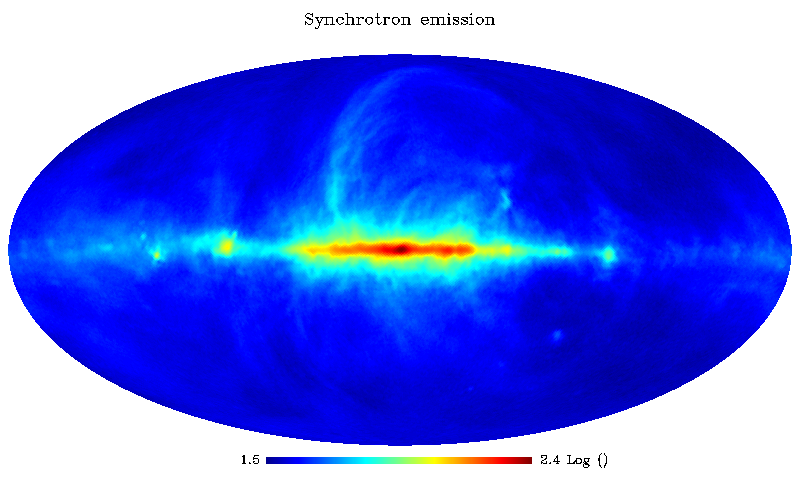
\includegraphics[width=7.5cm]{fig_sync.png}%[width=6.5cm,height=3.9cm]
 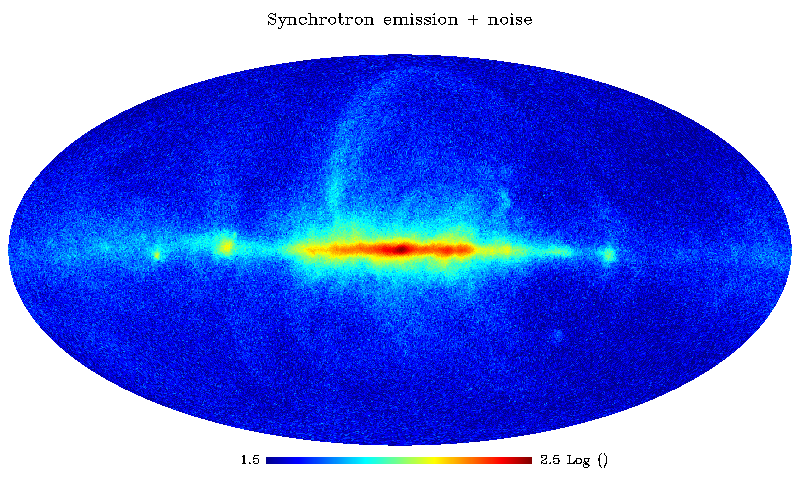
\includegraphics[width=7.5cm]{fig_sync_noise5.png}
}}
\centerline{
\hbox{
 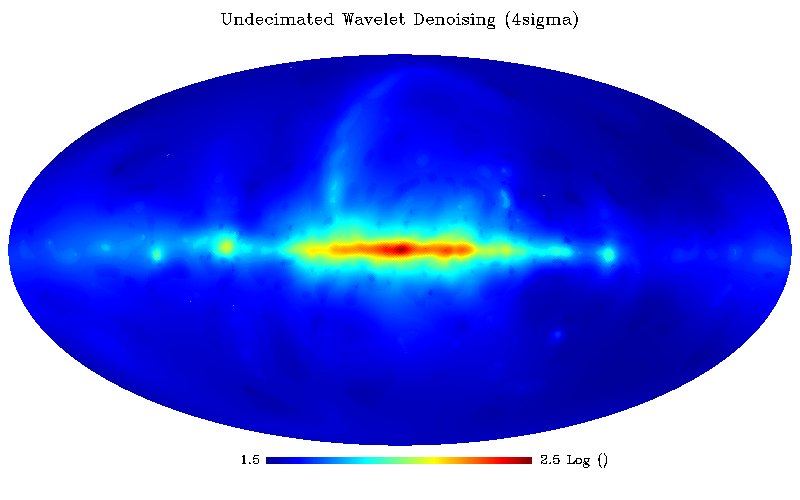
\includegraphics[width=7.5cm]{fig_sync_wtfilter5.png}
 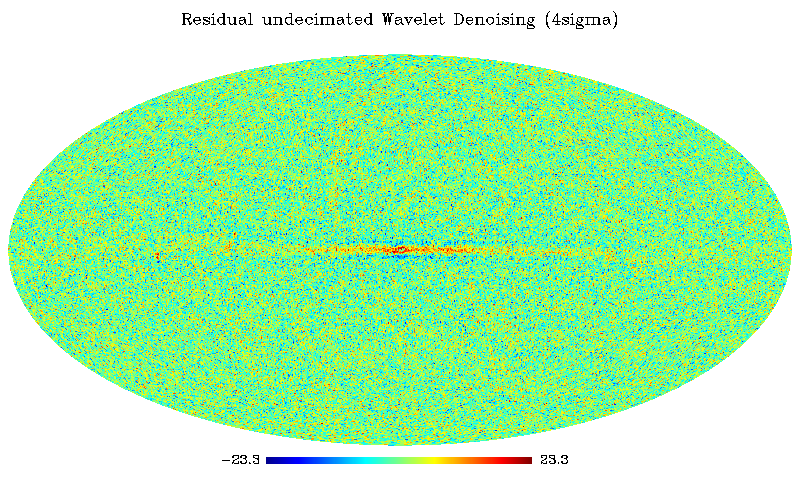
\includegraphics[width=7.5cm]{fig_sync_resi_wtfilter5.png}
}}
\centerline{
\hbox{
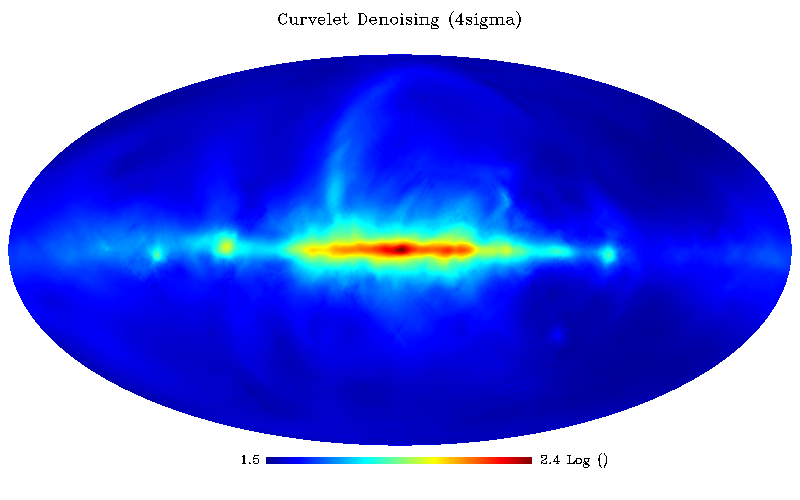
\includegraphics[width=7.5cm]{fig_sync_curfilter5.png}
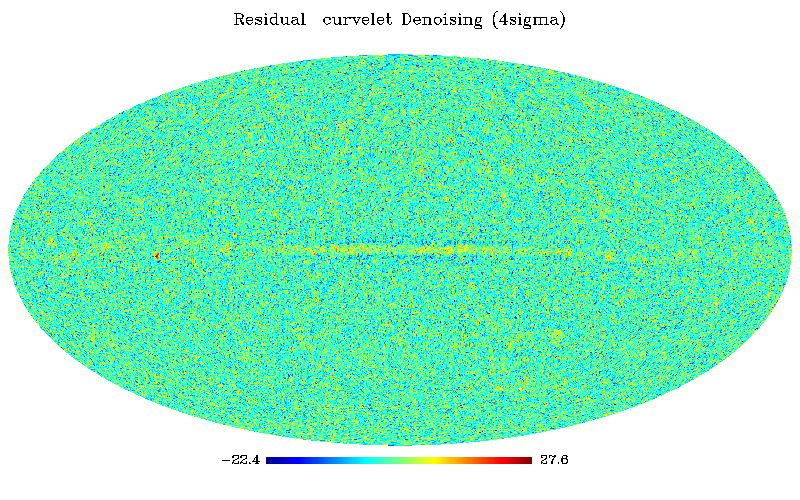
\includegraphics[width=7.5cm]{fig_sync_resi_curfilter5.png}
}}
}
 \caption{Denoising. Upper left and right: simulated 
synchrotron image and same image with
additive Gaussian noise (i.e.\ simulated data).  Middle: undecimated 
wavelet filtering and residual.
Bottom: pyramidal curvelet filtering  and residual.}
\label{Figure:sync_filter}
\index{data!synchrotron}
\end{figure}

\newpage
Fig.~\ref{Figure:sync_filter} describes the setting and the results of a simulated denoising experiment: 
upper left, the original simulated map of the  astrophysical synchrotron emission; upper right, the same image 
plus additive Gaussian noise ($\sigma=5$). Since the synchrotron image has a standard deviation (after renormalization) 
equal to $16.26$, the SNR is around  $3.25$.  The middle panels in this figure show the UWTS denoised image 
and the residuals. The bottom panels show the pyramidal curvelet transform filtered image and the residuals. 
On such data, exhibiting very anisotropic features, the curvelets produce better results than wavelets.

Although the results obtained by simply thresholding the curvelet expansion are encouraging, there is of course ample room for further
improvement. A quick inspection of the residual images for both the wavelet and curvelet transforms shown in Figure~\ref{Figure:sync_filter}
reveals the existence of very different features. For instance, wavelets do not restore long features with high fidelity while curvelets
are seriously challenged by isotropic or small features. Each transform has its own area of expertise and this complementarity is of great 
potential. The Combined Filtering Method (CFM) \citep{starck:spie01a} allows us to benefit from the advantages of both transforms. This iterative 
method detects the significant coefficients in both the wavelet domain and the curvelet domain and guarantees that the reconstructed map will 
take into account any pattern which is detected as significant by either of the transforms. 

\section{The Combined Filtering Method on the Sphere}
\index{wavelet!combined filtering}
\index{curvelet!combined filtering}
\index{combined filtering method}


In general, suppose that we are given $K$ linear transforms $T_1,
\ldots, T_K$ and let $\alpha_k$ be the coefficient sequence of an
object $x$ after applying the transform $T_k$, i.e. $\alpha_k = T_k
x$. We will assume that for each transform $T_k$ we have available a
reconstruction rule that we will denote by $T^{-1}_k$ although this is
clearly an abuse of notation.  Finally, $T$ will denote the block
diagonal matrix with the $T_k$'s as building blocks and $\alpha$ the
amalgamation of the $\alpha_k$'s.

A hard thresholding rule associated with the transform $T_k$ synthesizes 
an estimate $\tilde{s}_k$ via the formula 
\begin{equation}
\label{eq:ht}
\tilde{s}_k = T_k^{-1} \delta(\alpha_k)
\end{equation}
where $\delta$ is a rule that sets to zero all the coordinates of
$\alpha_k$ whose absolute value falls below a given sequence of
thresholds (such coordinates are said to be non-significant).\\
 
Given data $y$ of the form $y = s + \sigma z$, where $s$ is the image
we wish to recover and $z$ is standard white noise, we propose solving
the following optimization problem \citep{starck:spie01a}:
\begin{equation}
  \label{eq:l1-min}
  \min \|T\tilde{s}\|_{\ell_1}, \quad \mbox{subject to} \quad s \in C,  
\end{equation}
where $C$ is the set of vectors $\tilde{s}$ 
which obey the linear constraints
\begin{equation}
\label{eq:constraints}
\left\{  \begin{array}{ll}
  \tilde{s} \ge 0, \\
  |T\tilde{s} - Ty| \le e; 
  \end{array}
  \right. 
\end{equation}
here, the second inequality constraint 
only concerns the set of significant coefficients, 
i.e. those indices $\mu$ such that $\alpha_\mu =
(Ty)_\mu$ exceeds (in absolute value) a threshold $t_\mu$. Given a
vector of tolerance $(e_\mu)$, we seek a solution whose coefficients
  $(T\tilde{s})_\mu$ are within $e_\mu$ of the noisy
empirical $\alpha_\mu$'s.  Think of $\alpha_\mu$ as being given by
\[
y = \langle y, \varphi_\mu \rangle, 
\]
so that $\alpha_\mu$ is normally distributed with mean $\langle f,
\varphi_\mu \rangle$ and variance $\sigma^2_\mu = \sigma^2
\|\varphi_\mu\|^2_2$. In practice, the threshold values range
typically between three and four times the noise level $\sigma_\mu$
and in our experiments we will put $e_\mu = \sigma_\mu/2$. In short,
our constraints guarantee that the reconstruction will take into
account any pattern which is detected as significant by  any of the
$K$ transforms.
   
\subsection{The Minimization Method}

We propose solving \eqref{eq:l1-min} using the method of hybrid steepest descent (HSD) \citep{wave:yamada01}. 
HSD consists of building the sequence
\begin{eqnarray}
 s^{n+1} = P(s^{n}) - \lambda_{n+1} \nabla_J(P(s^{n})); 
\end{eqnarray}
Here, $P$ is the $\ell_2$ projection operator onto the feasible set $C$, $\nabla_J$ is the gradient of equation~\eqref{eq:l1-min}, 
and $(\lambda_{n})_{n \ge 1}$ is a sequence obeying $(\lambda_{n})_{n\ge 1} \in [0,1] $ and $\lim_{ n \rightarrow + \infty } \lambda_{n} = 0$.\\ \\
Algorothm~\ref{algo_cb_filter} gives the resulting combined filtering method.

%The combined filtering algorithm is:
%\begin{enumerate}
%\baselineskip=0.4truecm
%\itemsep=0.1truecm
%\item Initialize $L_{\max} = 1$, the number of iterations $N_i$, and
%  $\delta_{\lambda} = \frac{L_{\max}}{N_i}$.
%\item Estimate the noise standard deviation $\sigma$, and set $e_k =
%  \frac{\sigma}{2}$.
%\item For k = 1, .., $K$ calculate the transform: $\alpha^{(s)}_k
%  = T_k s$.
%\item Set $\lambda = L_{\max}$, $n = 0$, and $\tilde s^{n}$ to 0.
%\item While $\lambda >= 0$ do
%\begin{itemize}
%\item $u = \tilde s^{n}$.
%\item For k = 1, .., $K$ do
%  \begin{itemize}
%  \item Calculate the transform $\alpha_{k} = T_k u$.
%  \item For all coefficients $\alpha_{k,l}$ do
%     \begin{itemize}
%     \item Calculate the residual $r_{k,l} = \alpha^{(s)}_{k,l} -
%       \alpha_{k,l}$
%       
%     \item if $\alpha^{(s)}_{k,l}$ is significant and $ \mid r_{k,l}
%       \mid > e_{k,l}$ then $\alpha_{k,l} = \alpha^{(s)}_{k,l}$
%     \item $\alpha_{k,l} = sgn(\alpha_{k,l}) ( \mid \alpha_{k,l} \mid - \lambda)_{+}$.
%     \end{itemize}
%   \item $u = T_k^{-1} \alpha_{k}$
%  \end{itemize}
%\item Threshold negative values in $u$ and $\tilde s^{n+1} = u$.
%\item $n = n + 1$, $\lambda = \lambda - \delta_{\lambda} $, and goto 5.
%\end{itemize}
%\end{enumerate}

{\linespread{1}
\begin{algorithm}[h]
\caption{The combined filtering on the Sphere.}
\label{algo_cb_filter}
\noindent{\bf Task:} Compute the combined filtering on the sphere of a discrete $s$.\\
\noindent{\bf Parameters:} Data samples $s$, number of iterations $N_i$ and number of selected transforms $K$.\\
\noindent{\bf Initialization:}
\begin{itemize}
\item $L_{\max} = 1$
\item $\delta_{\lambda} = \frac{L_{\max}}{N_i}$
\item Estimate the noise standard deviation $\sigma$, and set $e_k = \frac{\sigma}{2}$.
\item \lFor{$k = 1, \ldots, K$}{calculate the transform: $\alpha^{(s)}_k = T_k s$.}
\item Set $\lambda = L_{\max}$, $n = 0$, and $\tilde s^{n}$ to 0.
\end{itemize}
\While{$\lambda >= 0$}{
	\begin{enumerate}[1.]
	\item $u = \tilde s^{n}$.
	\item \For{$k = 1, \ldots, K$}{
		\begin{itemize}
		\item Calculate the transform $\alpha_{k} = T_k u$.
		%\item For all coefficients $\alpha_{k,l}$ do
		\item \ForEach{$\alpha_{k,l}$}{
			\begin{itemize}
			\item Calculate the residual $r_{k,l} = \alpha^{(s)}_{k,l} - \alpha_{k,l}$
			%\item if $\alpha^{(s)}_{k,l}$ is significant and $ \mid r_{k,l} \mid > e_{k,l}$ then $\alpha_{k,l} = \alpha^{(s)}_{k,l}$
			\item \lIf{ $\alpha^{(s)}_{k,l}$ is significant AND $ \mid r_{k,l} \mid > e_{k,l}$ }{$\alpha_{k,l} = \alpha^{(s)}_{k,l}$}
			\item $\alpha_{k,l} = sgn(\alpha_{k,l}) ( \mid \alpha_{k,l} \mid - \lambda)_{+}$.
			\end{itemize}
			}%end foreach
		\item $u = T_k^{-1} \alpha_{k}$
		\end{itemize}	
		}%end for k
	\item Threshold negative values in $u$ and $\tilde s^{n+1} = u$.
	\item $n = n + 1$, $\lambda = \lambda - \delta_{\lambda}$
	\end{enumerate}
}%end while
\noindent{\bf Output:} $\tilde s^{m}$ with $m = N_i$, filtered map.
\end{algorithm}
}

\begin{figure}[htb]
\vbox{
\centerline{
\hbox{
 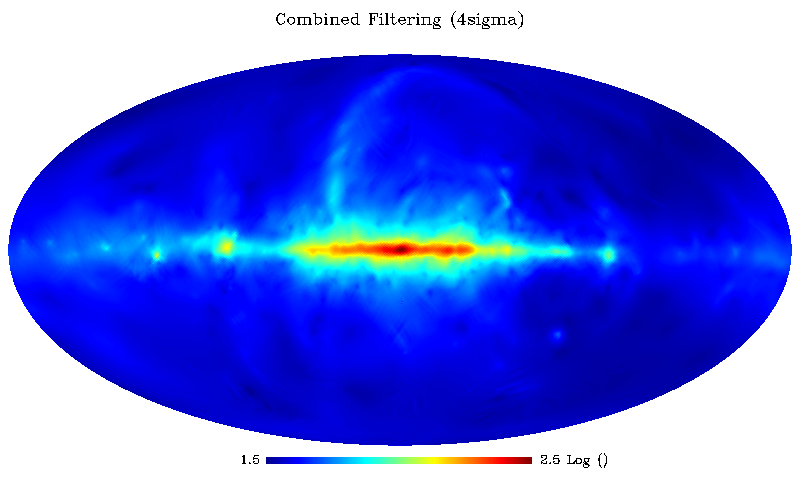
\includegraphics[width=12cm]{fig_sync_cbfilter5.png}
 }}
 \centerline{
 \hbox{
 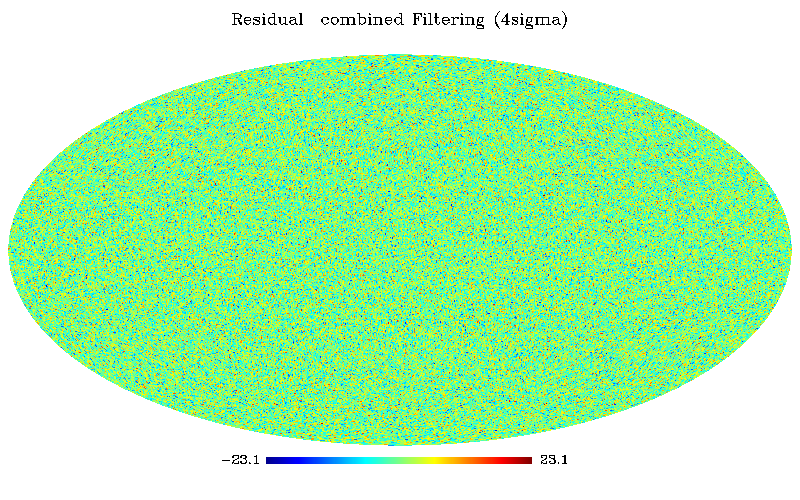
\includegraphics[width=12cm]{fig_sync_resi_cbfilter5.png}
}}}
 \caption{Combined denoising (using both wavelets and curvelets) and residuals.}
\label{Figure:sync_cbf_filter}
\index{data!synchrotron}
\end{figure}

\begin{table}[htb]
\baselineskip=0.4cm
\begin{center}
\begin{tabular}{lcccc} \hline \hline
Method                          &  Error standard deviation       \\ \hline \hline
Noisy map                       & 5    8  \\
Wavelet                         & 1.25     \\
Curvelet                        & 1.07   \\
CFA                             & 0.86  \\ \hline
\hline
\end{tabular}
\caption{Error standard deviations after denoising the synchrotron noisy map (additive white Gaussian noise, $\sigma = 5$) by the wavelet, the curvelet and the combined denoising algorithm.}
\label{comptab_sync}
\end{center}
\end{table}

 
\begin{figure}
\centerline{
\hbox{
 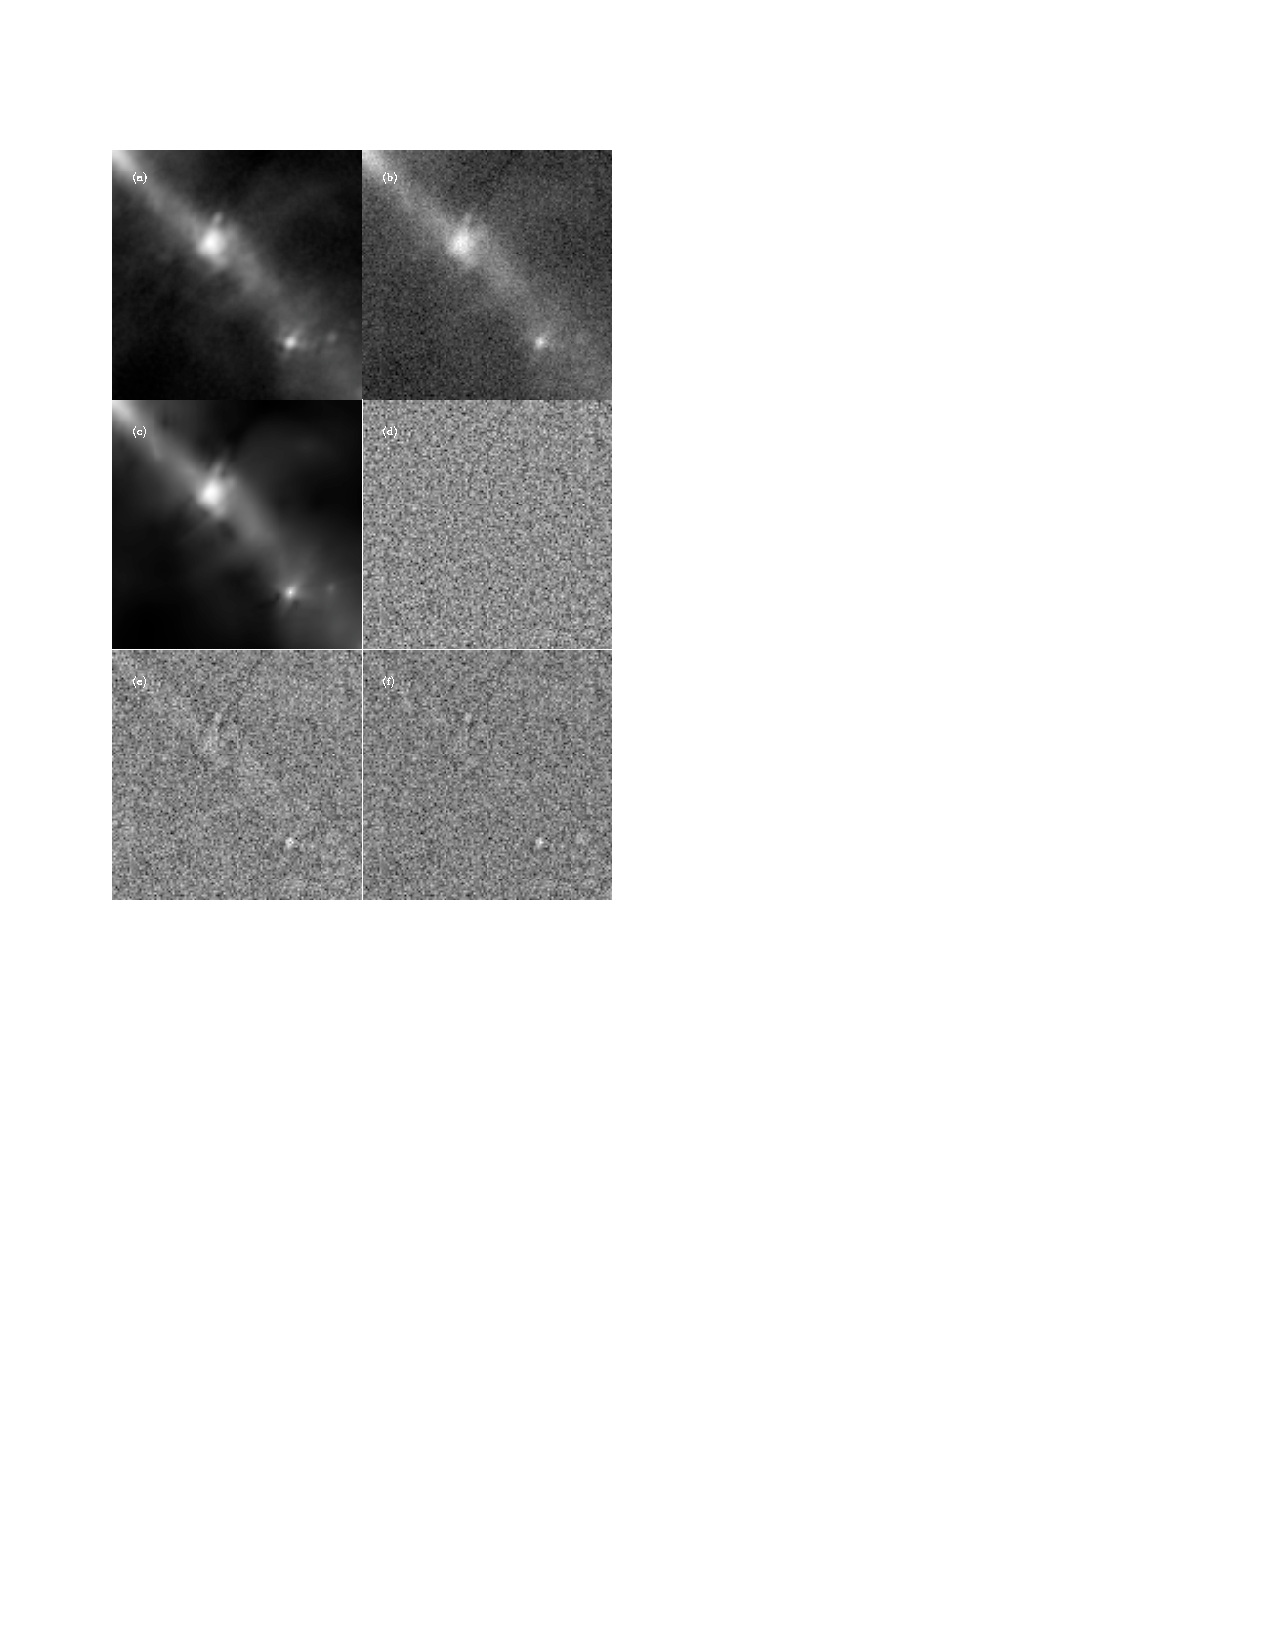
\includegraphics[trim= 1cm 12cm 10cm 2cm, width=\textwidth]{fig_cmp_fil_synchrotron_face6_bw.pdf}
 }}
\caption{Combined Filtering Method, face 6 in the Healpix representation of the image shown in figure~\ref{Figure:sync_cbf_filter}. 
From top to bottom and left to right, respectively the a) original image face, b) the noisy image, c) the combined filtered image, 
d) the combined filtering residual, e) the wavelet filtering residual and f) the curvelet filtering residual.}
\label{Figure:sync_face_cbf_filter}
\end{figure}
 
\subsection{Experiments}
Figure~\ref{Figure:sync_cbf_filter} shows the CFM denoised image and its residual. { Figure~\ref{Figure:sync_face_cbf_filter} shows one face 
(face 6) of the following Healpix images: upper left, original image; upper right, noisy image; middle left, restored image after denoising 
by the combined transform; middle right, the residual; bottom left and right, the residual using respectively the curvelet and the wavelet 
denoising method. } The results are reported in Table~\ref{comptab_sync}. The residual is much better when the combined filtering is applied, 
and no feature can be detected any more by eye in the residual. This was not the case for either the wavelet and the curvelet filtering.
 
 
 